\section{Requirements Elicitation - ''Anforderungserhebung''}
\begin{itemize}
	\item Prozess des \textit{Suchens, Aufdeckens, Erwerbens, Ausarbeiten} von R für computerbasierte Systeme
	\item Teil der frühen Entwicklungsphase, aber fortlaufend und kritisch
	\item komplex, verschiedenste Techniken - vor allem aus Sozialwissenschaften - finden Anwendung
	\begin{itemize}
		\item großer Problemfaktor liegt in Kommunikation zw. Engineers und Kunde
		\item Iterative Erarbeitung, setzt stark auf Kommunikationskills der Engineers und Bereitschaft der Stakeholder
		\item Problem: Konzepte, die für A verständlich sind, könnten für B komplett unverständlich sein
	\end{itemize}
	\item Probleme der Erhebung
	\begin{itemize}
		\item Scope: Systemgrenzen sind falsch definiert; unnötige technische Details spezifiziert, die eher verwirren als helfen
		\item Understanding: Kunde weiß nicht genau was er will; was seine Computer-Umgebung her gibt; versteht das Problem nicht ganz; Lässt Infos aus die ''offensichtlich'' sind0
		\item Flüchtigkeit: R verändern sich mit der Zeit
	\end{itemize}
\end{itemize}
5 Fundamentale Aktivitäten zur Erhebung
\begin{enumerate}
	\item Verstehen der Anwendungsdomäne\\
	Beschreibung existierender Arbeitsprozesse und die zugehörigen Probleme, die vom System gelöst werden sollen.
	\item Quellen der R identifizieren\\
	verschiedenste Quellen -> Stakeholder (meistens); Existierende Systeme und Prozesse; exist. Doku über aktuelles System und Prozesse
	\item Analyse Stakeholder\\
	Identifizieren wer der ''offensichtlichste'' Stakeholder ist -> mal der Endkunde, mal der Geldgeber etc
	\item Methoden, Ansätze, Tools auswählen\\
	Gründe für Methodenauswahl: einzige, die der Analyst kennt; sein Favorit; vorgeschrieben;...
	\item R erheben von Stakeholder und anderen Quellen\\
	Ergebnis = detaillierte Menge von R in natürlicher Sprache und einfachen Diagrammen
\end{enumerate}
\begin{figure}[!h]
	\centering
	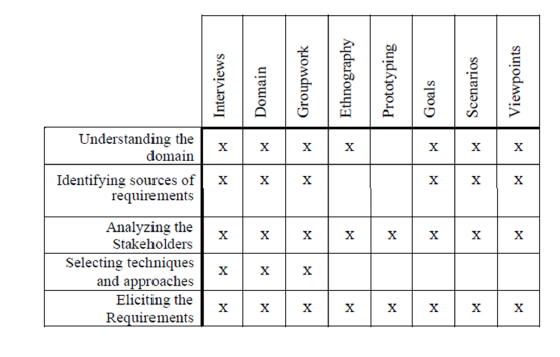
\includegraphics[scale=0.6]{img/elicitation_techniques.png}
	\caption{Which techniques and approaches should be used for a given
		requirements elicitation activity?}
\end{figure}

Wir benötigen unterschiedliche Techniken, da jede Technik anderes Wissen als Ergebnis liefert.

\subsection{Techniken und Ansätze}
\subsubsection{Task Analysis and Domain Analysis}
Beschreibung der Aufgaben, Rollen und Aufgabendomain in der aktuell vorgestellten Situation.\\
\textbf{Task Modeling}
\begin{itemize}
	\item \textit{Hierarchisches Beschreibung} in  SubTasks und deren Beschreibung
	\item Tasks werden ausgeführt um ein Ziel zu erreichen; meist von Actor in bestimmter Rolle
	\item Alternative: \textit{Temporale Beschreibung} 
\end{itemize}
\textbf{Task Domain}\\
oft objektorientiert modelliert\\
\\
Wurzel eines Task Models ist ein Use Case\\
\\
\textbf{Analysis Synthesis Bridge Model}
\begin{figure}[!h]
	\centering
	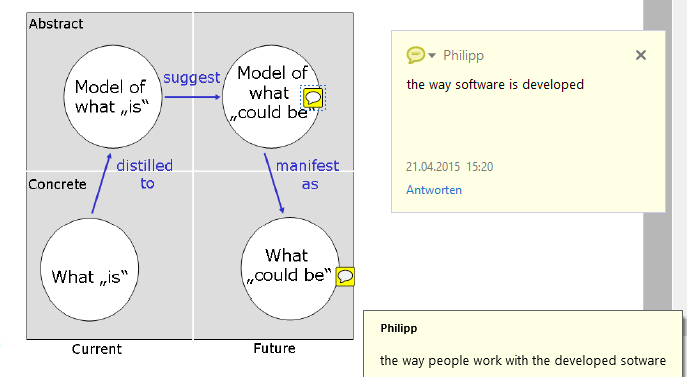
\includegraphics[scale=0.6]{img/analysis_synthesis_bridge_model.png}
	\caption{Analysis Synthesis Bridge Model}
\end{figure}

\subsubsection{Repertory Grids}
\begin{itemize}
	\item liefert impliziertes Wissen
	\item basiert auf den persönlichen Konstrukten eines Individuums, in denen die Interaktion mit anderen eingeordnet wird -> hat Einfluss auf die weitere Interaktion mit anderen Menschen
	\item Zuordnung von Werten zu einer Domain Entität\\
	Ergebnis => System wird als Matrix modelliert bei der die Elemente des Systems kategorisiert werden
	\item Ziel ist das Identifizieren von Unterschieden und Gemeinsamkeiten zwischen den einzelnen Domainbereichen
\end{itemize}

\subsubsection{Interviews}
\begin{itemize}
	\item meist verbreitet und oft eingesetzt
	\item Human Based social Activity -> eher informal und Ergebnis hängt stark vom Zsmspiel der Beteiligten ab
	\item große Datenmenge in kurzer Zeit mgl
	\item 3 Arten:
	\begin{itemize}
		\item unstructured: kein vordefinierter Ablauf von Fragen etc; oft eingesetzt wenn Domäne etc noch sehr unklar formuliert; Risiko das manche Themen komplett wegfallen
		\item semi-structured: Zwischending
		\item structured: vorgefertigter Fragenkatalog, der abgearbeitet wird; Erfolg hängt von den richtigen Fragen ab, wann und wem sie gestellt werden
	\end{itemize}
\end{itemize}